% Created by tikzDevice version 0.12.4 on 2023-07-06 13:18:27
% !TEX encoding = UTF-8 Unicode
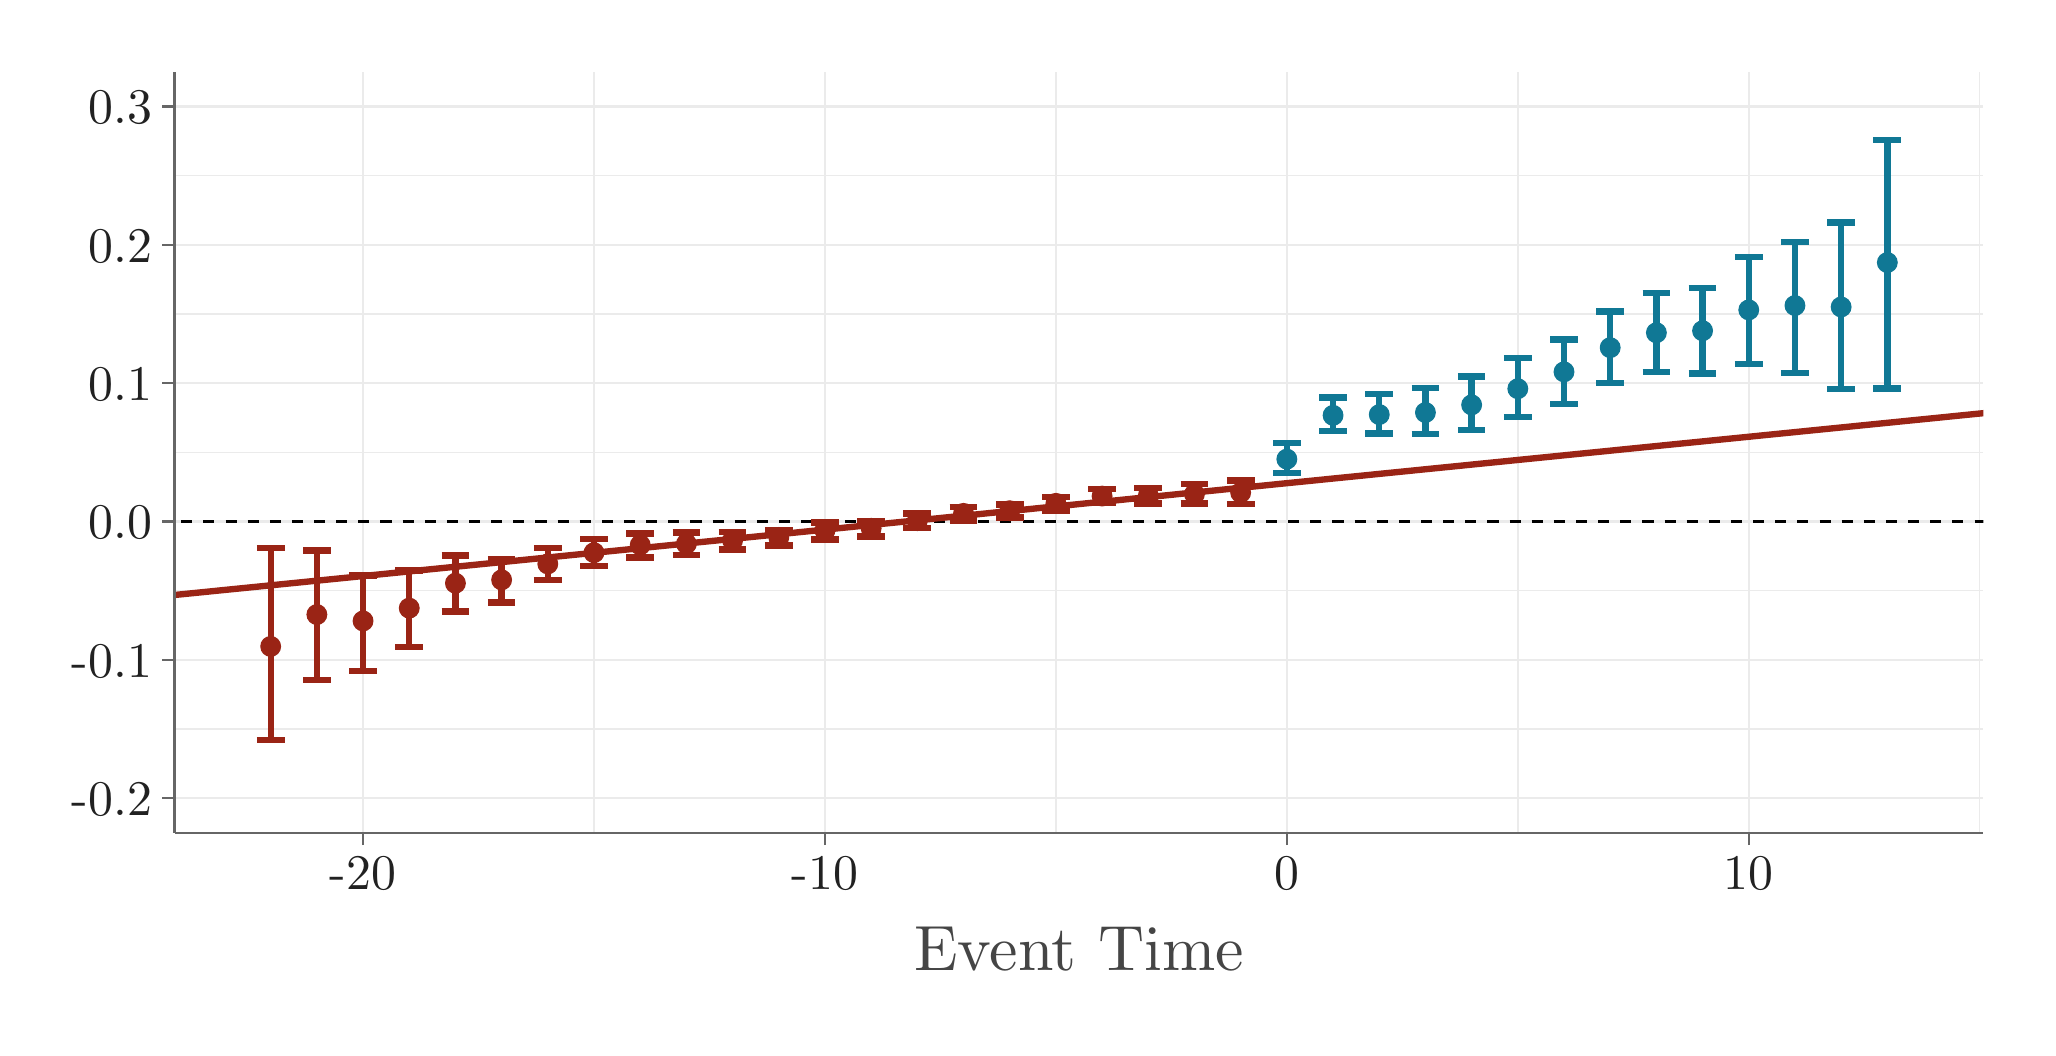
\begin{tikzpicture}[x=1pt,y=1pt]
\definecolor{fillColor}{RGB}{255,255,255}
\path[use as bounding box,fill=fillColor,fill opacity=0.00] (0,0) rectangle (722.70,361.35);
\begin{scope}
\path[clip] (  0.00,  0.00) rectangle (722.70,361.35);
\definecolor{fillColor}{RGB}{255,255,255}

\path[fill=fillColor] (  0.00, -0.00) rectangle (722.70,361.35);
\end{scope}
\begin{scope}
\path[clip] ( 53.09, 70.42) rectangle (706.70,345.35);
\definecolor{fillColor}{RGB}{255,255,255}

\path[fill=fillColor] ( 53.09, 70.42) rectangle (706.70,345.35);
\definecolor{drawColor}{gray}{0.92}

\path[draw=drawColor,line width= 0.5pt,line join=round] ( 53.09,107.91) --
	(706.70,107.91);

\path[draw=drawColor,line width= 0.5pt,line join=round] ( 53.09,157.90) --
	(706.70,157.90);

\path[draw=drawColor,line width= 0.5pt,line join=round] ( 53.09,207.89) --
	(706.70,207.89);

\path[draw=drawColor,line width= 0.5pt,line join=round] ( 53.09,257.87) --
	(706.70,257.87);

\path[draw=drawColor,line width= 0.5pt,line join=round] ( 53.09,307.86) --
	(706.70,307.86);

\path[draw=drawColor,line width= 0.5pt,line join=round] (204.64, 70.42) --
	(204.64,345.35);

\path[draw=drawColor,line width= 0.5pt,line join=round] (371.55, 70.42) --
	(371.55,345.35);

\path[draw=drawColor,line width= 0.5pt,line join=round] (538.46, 70.42) --
	(538.46,345.35);

\path[draw=drawColor,line width= 0.5pt,line join=round] (705.36, 70.42) --
	(705.36,345.35);

\path[draw=drawColor,line width= 0.9pt,line join=round] ( 53.09, 82.92) --
	(706.70, 82.92);

\path[draw=drawColor,line width= 0.9pt,line join=round] ( 53.09,132.91) --
	(706.70,132.91);

\path[draw=drawColor,line width= 0.9pt,line join=round] ( 53.09,182.89) --
	(706.70,182.89);

\path[draw=drawColor,line width= 0.9pt,line join=round] ( 53.09,232.88) --
	(706.70,232.88);

\path[draw=drawColor,line width= 0.9pt,line join=round] ( 53.09,282.87) --
	(706.70,282.87);

\path[draw=drawColor,line width= 0.9pt,line join=round] ( 53.09,332.85) --
	(706.70,332.85);

\path[draw=drawColor,line width= 0.9pt,line join=round] (121.19, 70.42) --
	(121.19,345.35);

\path[draw=drawColor,line width= 0.9pt,line join=round] (288.10, 70.42) --
	(288.10,345.35);

\path[draw=drawColor,line width= 0.9pt,line join=round] (455.00, 70.42) --
	(455.00,345.35);

\path[draw=drawColor,line width= 0.9pt,line join=round] (621.91, 70.42) --
	(621.91,345.35);
\definecolor{drawColor}{RGB}{0,0,0}

\path[draw=drawColor,line width= 0.9pt,dash pattern=on 4pt off 4pt ,line join=round] (-600.51,182.89) -- (1360.31,182.89);
\definecolor{drawColor}{RGB}{154,36,21}

\path[draw=drawColor,line width= 2.3pt,line join=round] (-600.51, 90.65) -- (1360.31,287.75);
\definecolor{fillColor}{RGB}{154,36,21}

\path[draw=drawColor,line width= 0.4pt,line join=round,line cap=round,fill=fillColor] ( 87.81,137.76) circle (  3.57);

\path[draw=drawColor,line width= 0.4pt,line join=round,line cap=round,fill=fillColor] (104.50,149.28) circle (  3.57);

\path[draw=drawColor,line width= 0.4pt,line join=round,line cap=round,fill=fillColor] (121.19,146.96) circle (  3.57);

\path[draw=drawColor,line width= 0.4pt,line join=round,line cap=round,fill=fillColor] (137.88,151.60) circle (  3.57);

\path[draw=drawColor,line width= 0.4pt,line join=round,line cap=round,fill=fillColor] (154.57,160.61) circle (  3.57);

\path[draw=drawColor,line width= 0.4pt,line join=round,line cap=round,fill=fillColor] (171.26,161.80) circle (  3.57);

\path[draw=drawColor,line width= 0.4pt,line join=round,line cap=round,fill=fillColor] (187.95,167.58) circle (  3.57);

\path[draw=drawColor,line width= 0.4pt,line join=round,line cap=round,fill=fillColor] (204.64,171.64) circle (  3.57);

\path[draw=drawColor,line width= 0.4pt,line join=round,line cap=round,fill=fillColor] (221.34,174.40) circle (  3.57);

\path[draw=drawColor,line width= 0.4pt,line join=round,line cap=round,fill=fillColor] (238.03,174.85) circle (  3.57);

\path[draw=drawColor,line width= 0.4pt,line join=round,line cap=round,fill=fillColor] (254.72,176.06) circle (  3.57);

\path[draw=drawColor,line width= 0.4pt,line join=round,line cap=round,fill=fillColor] (271.41,177.16) circle (  3.57);

\path[draw=drawColor,line width= 0.4pt,line join=round,line cap=round,fill=fillColor] (288.10,179.67) circle (  3.57);

\path[draw=drawColor,line width= 0.4pt,line join=round,line cap=round,fill=fillColor] (304.79,180.44) circle (  3.57);

\path[draw=drawColor,line width= 0.4pt,line join=round,line cap=round,fill=fillColor] (321.48,183.21) circle (  3.57);

\path[draw=drawColor,line width= 0.4pt,line join=round,line cap=round,fill=fillColor] (338.17,185.84) circle (  3.57);

\path[draw=drawColor,line width= 0.4pt,line join=round,line cap=round,fill=fillColor] (354.86,186.81) circle (  3.57);

\path[draw=drawColor,line width= 0.4pt,line join=round,line cap=round,fill=fillColor] (371.55,189.47) circle (  3.57);

\path[draw=drawColor,line width= 0.4pt,line join=round,line cap=round,fill=fillColor] (388.24,192.09) circle (  3.57);

\path[draw=drawColor,line width= 0.4pt,line join=round,line cap=round,fill=fillColor] (404.93,192.19) circle (  3.57);

\path[draw=drawColor,line width= 0.4pt,line join=round,line cap=round,fill=fillColor] (421.62,192.81) circle (  3.57);

\path[draw=drawColor,line width= 0.4pt,line join=round,line cap=round,fill=fillColor] (438.31,193.33) circle (  3.57);
\definecolor{drawColor}{RGB}{16,120,149}
\definecolor{fillColor}{RGB}{16,120,149}

\path[draw=drawColor,line width= 0.4pt,line join=round,line cap=round,fill=fillColor] (455.00,205.45) circle (  3.57);

\path[draw=drawColor,line width= 0.4pt,line join=round,line cap=round,fill=fillColor] (471.70,221.26) circle (  3.57);

\path[draw=drawColor,line width= 0.4pt,line join=round,line cap=round,fill=fillColor] (488.39,221.54) circle (  3.57);

\path[draw=drawColor,line width= 0.4pt,line join=round,line cap=round,fill=fillColor] (505.08,222.28) circle (  3.57);

\path[draw=drawColor,line width= 0.4pt,line join=round,line cap=round,fill=fillColor] (521.77,225.04) circle (  3.57);

\path[draw=drawColor,line width= 0.4pt,line join=round,line cap=round,fill=fillColor] (538.46,230.89) circle (  3.57);

\path[draw=drawColor,line width= 0.4pt,line join=round,line cap=round,fill=fillColor] (555.15,236.97) circle (  3.57);

\path[draw=drawColor,line width= 0.4pt,line join=round,line cap=round,fill=fillColor] (571.84,245.72) circle (  3.57);

\path[draw=drawColor,line width= 0.4pt,line join=round,line cap=round,fill=fillColor] (588.53,251.11) circle (  3.57);

\path[draw=drawColor,line width= 0.4pt,line join=round,line cap=round,fill=fillColor] (605.22,251.82) circle (  3.57);

\path[draw=drawColor,line width= 0.4pt,line join=round,line cap=round,fill=fillColor] (621.91,259.36) circle (  3.57);

\path[draw=drawColor,line width= 0.4pt,line join=round,line cap=round,fill=fillColor] (638.60,260.94) circle (  3.57);

\path[draw=drawColor,line width= 0.4pt,line join=round,line cap=round,fill=fillColor] (655.29,260.42) circle (  3.57);

\path[draw=drawColor,line width= 0.4pt,line join=round,line cap=round,fill=fillColor] (671.98,276.48) circle (  3.57);
\definecolor{drawColor}{RGB}{154,36,21}

\path[draw=drawColor,line width= 2.3pt,line join=round] ( 82.80,173.29) --
	( 92.82,173.29);

\path[draw=drawColor,line width= 2.3pt,line join=round] ( 87.81,173.29) --
	( 87.81,103.86);

\path[draw=drawColor,line width= 2.3pt,line join=round] ( 82.80,103.86) --
	( 92.82,103.86);

\path[draw=drawColor,line width= 2.3pt,line join=round] ( 99.49,172.40) --
	(109.51,172.40);

\path[draw=drawColor,line width= 2.3pt,line join=round] (104.50,172.40) --
	(104.50,125.71);

\path[draw=drawColor,line width= 2.3pt,line join=round] ( 99.49,125.71) --
	(109.51,125.71);

\path[draw=drawColor,line width= 2.3pt,line join=round] (116.18,163.45) --
	(126.20,163.45);

\path[draw=drawColor,line width= 2.3pt,line join=round] (121.19,163.45) --
	(121.19,128.99);

\path[draw=drawColor,line width= 2.3pt,line join=round] (116.18,128.99) --
	(126.20,128.99);

\path[draw=drawColor,line width= 2.3pt,line join=round] (132.87,165.16) --
	(142.89,165.16);

\path[draw=drawColor,line width= 2.3pt,line join=round] (137.88,165.16) --
	(137.88,137.59);

\path[draw=drawColor,line width= 2.3pt,line join=round] (132.87,137.59) --
	(142.89,137.59);

\path[draw=drawColor,line width= 2.3pt,line join=round] (149.57,170.66) --
	(159.58,170.66);

\path[draw=drawColor,line width= 2.3pt,line join=round] (154.57,170.66) --
	(154.57,150.33);

\path[draw=drawColor,line width= 2.3pt,line join=round] (149.57,150.33) --
	(159.58,150.33);

\path[draw=drawColor,line width= 2.3pt,line join=round] (166.26,169.14) --
	(176.27,169.14);

\path[draw=drawColor,line width= 2.3pt,line join=round] (171.26,169.14) --
	(171.26,153.60);

\path[draw=drawColor,line width= 2.3pt,line join=round] (166.26,153.60) --
	(176.27,153.60);

\path[draw=drawColor,line width= 2.3pt,line join=round] (182.95,173.29) --
	(192.96,173.29);

\path[draw=drawColor,line width= 2.3pt,line join=round] (187.95,173.29) --
	(187.95,161.73);

\path[draw=drawColor,line width= 2.3pt,line join=round] (182.95,161.73) --
	(192.96,161.73);

\path[draw=drawColor,line width= 2.3pt,line join=round] (199.64,176.49) --
	(209.65,176.49);

\path[draw=drawColor,line width= 2.3pt,line join=round] (204.64,176.49) --
	(204.64,166.75);

\path[draw=drawColor,line width= 2.3pt,line join=round] (199.64,166.75) --
	(209.65,166.75);

\path[draw=drawColor,line width= 2.3pt,line join=round] (216.33,178.53) --
	(226.34,178.53);

\path[draw=drawColor,line width= 2.3pt,line join=round] (221.34,178.53) --
	(221.34,169.89);

\path[draw=drawColor,line width= 2.3pt,line join=round] (216.33,169.89) --
	(226.34,169.89);

\path[draw=drawColor,line width= 2.3pt,line join=round] (233.02,178.96) --
	(243.03,178.96);

\path[draw=drawColor,line width= 2.3pt,line join=round] (238.03,178.96) --
	(238.03,170.80);

\path[draw=drawColor,line width= 2.3pt,line join=round] (233.02,170.80) --
	(243.03,170.80);

\path[draw=drawColor,line width= 2.3pt,line join=round] (249.71,179.04) --
	(259.72,179.04);

\path[draw=drawColor,line width= 2.3pt,line join=round] (254.72,179.04) --
	(254.72,172.77);

\path[draw=drawColor,line width= 2.3pt,line join=round] (249.71,172.77) --
	(259.72,172.77);

\path[draw=drawColor,line width= 2.3pt,line join=round] (266.40,179.92) --
	(276.41,179.92);

\path[draw=drawColor,line width= 2.3pt,line join=round] (271.41,179.92) --
	(271.41,174.21);

\path[draw=drawColor,line width= 2.3pt,line join=round] (266.40,174.21) --
	(276.41,174.21);

\path[draw=drawColor,line width= 2.3pt,line join=round] (283.09,182.48) --
	(293.10,182.48);

\path[draw=drawColor,line width= 2.3pt,line join=round] (288.10,182.48) --
	(288.10,176.43);

\path[draw=drawColor,line width= 2.3pt,line join=round] (283.09,176.43) --
	(293.10,176.43);

\path[draw=drawColor,line width= 2.3pt,line join=round] (299.78,183.15) --
	(309.80,183.15);

\path[draw=drawColor,line width= 2.3pt,line join=round] (304.79,183.15) --
	(304.79,177.44);

\path[draw=drawColor,line width= 2.3pt,line join=round] (299.78,177.44) --
	(309.80,177.44);

\path[draw=drawColor,line width= 2.3pt,line join=round] (316.47,185.82) --
	(326.49,185.82);

\path[draw=drawColor,line width= 2.3pt,line join=round] (321.48,185.82) --
	(321.48,180.50);

\path[draw=drawColor,line width= 2.3pt,line join=round] (316.47,180.50) --
	(326.49,180.50);

\path[draw=drawColor,line width= 2.3pt,line join=round] (333.16,188.22) --
	(343.18,188.22);

\path[draw=drawColor,line width= 2.3pt,line join=round] (338.17,188.22) --
	(338.17,183.28);

\path[draw=drawColor,line width= 2.3pt,line join=round] (333.16,183.28) --
	(343.18,183.28);

\path[draw=drawColor,line width= 2.3pt,line join=round] (349.85,189.08) --
	(359.87,189.08);

\path[draw=drawColor,line width= 2.3pt,line join=round] (354.86,189.08) --
	(354.86,184.31);

\path[draw=drawColor,line width= 2.3pt,line join=round] (349.85,184.31) --
	(359.87,184.31);

\path[draw=drawColor,line width= 2.3pt,line join=round] (366.54,191.87) --
	(376.56,191.87);

\path[draw=drawColor,line width= 2.3pt,line join=round] (371.55,191.87) --
	(371.55,186.90);

\path[draw=drawColor,line width= 2.3pt,line join=round] (366.54,186.90) --
	(376.56,186.90);

\path[draw=drawColor,line width= 2.3pt,line join=round] (383.23,194.69) --
	(393.25,194.69);

\path[draw=drawColor,line width= 2.3pt,line join=round] (388.24,194.69) --
	(388.24,189.63);

\path[draw=drawColor,line width= 2.3pt,line join=round] (383.23,189.63) --
	(393.25,189.63);

\path[draw=drawColor,line width= 2.3pt,line join=round] (399.93,195.12) --
	(409.94,195.12);

\path[draw=drawColor,line width= 2.3pt,line join=round] (404.93,195.12) --
	(404.93,189.41);

\path[draw=drawColor,line width= 2.3pt,line join=round] (399.93,189.41) --
	(409.94,189.41);

\path[draw=drawColor,line width= 2.3pt,line join=round] (416.62,196.40) --
	(426.63,196.40);

\path[draw=drawColor,line width= 2.3pt,line join=round] (421.62,196.40) --
	(421.62,189.41);

\path[draw=drawColor,line width= 2.3pt,line join=round] (416.62,189.41) --
	(426.63,189.41);

\path[draw=drawColor,line width= 2.3pt,line join=round] (433.31,197.73) --
	(443.32,197.73);

\path[draw=drawColor,line width= 2.3pt,line join=round] (438.31,197.73) --
	(438.31,189.15);

\path[draw=drawColor,line width= 2.3pt,line join=round] (433.31,189.15) --
	(443.32,189.15);
\definecolor{drawColor}{RGB}{16,120,149}

\path[draw=drawColor,line width= 2.3pt,line join=round] (450.00,211.17) --
	(460.01,211.17);

\path[draw=drawColor,line width= 2.3pt,line join=round] (455.00,211.17) --
	(455.00,200.37);

\path[draw=drawColor,line width= 2.3pt,line join=round] (450.00,200.37) --
	(460.01,200.37);

\path[draw=drawColor,line width= 2.3pt,line join=round] (466.69,227.65) --
	(476.70,227.65);

\path[draw=drawColor,line width= 2.3pt,line join=round] (471.70,227.65) --
	(471.70,215.50);

\path[draw=drawColor,line width= 2.3pt,line join=round] (466.69,215.50) --
	(476.70,215.50);

\path[draw=drawColor,line width= 2.3pt,line join=round] (483.38,229.06) --
	(493.39,229.06);

\path[draw=drawColor,line width= 2.3pt,line join=round] (488.39,229.06) --
	(488.39,214.72);

\path[draw=drawColor,line width= 2.3pt,line join=round] (483.38,214.72) --
	(493.39,214.72);

\path[draw=drawColor,line width= 2.3pt,line join=round] (500.07,231.23) --
	(510.08,231.23);

\path[draw=drawColor,line width= 2.3pt,line join=round] (505.08,231.23) --
	(505.08,214.41);

\path[draw=drawColor,line width= 2.3pt,line join=round] (500.07,214.41) --
	(510.08,214.41);

\path[draw=drawColor,line width= 2.3pt,line join=round] (516.76,235.32) --
	(526.77,235.32);

\path[draw=drawColor,line width= 2.3pt,line join=round] (521.77,235.32) --
	(521.77,215.95);

\path[draw=drawColor,line width= 2.3pt,line join=round] (516.76,215.95) --
	(526.77,215.95);

\path[draw=drawColor,line width= 2.3pt,line join=round] (533.45,241.93) --
	(543.47,241.93);

\path[draw=drawColor,line width= 2.3pt,line join=round] (538.46,241.93) --
	(538.46,220.75);

\path[draw=drawColor,line width= 2.3pt,line join=round] (533.45,220.75) --
	(543.47,220.75);

\path[draw=drawColor,line width= 2.3pt,line join=round] (550.14,248.71) --
	(560.16,248.71);

\path[draw=drawColor,line width= 2.3pt,line join=round] (555.15,248.71) --
	(555.15,225.46);

\path[draw=drawColor,line width= 2.3pt,line join=round] (550.14,225.46) --
	(560.16,225.46);

\path[draw=drawColor,line width= 2.3pt,line join=round] (566.83,258.74) --
	(576.85,258.74);

\path[draw=drawColor,line width= 2.3pt,line join=round] (571.84,258.74) --
	(571.84,232.91);

\path[draw=drawColor,line width= 2.3pt,line join=round] (566.83,232.91) --
	(576.85,232.91);

\path[draw=drawColor,line width= 2.3pt,line join=round] (583.52,265.53) --
	(593.54,265.53);

\path[draw=drawColor,line width= 2.3pt,line join=round] (588.53,265.53) --
	(588.53,236.92);

\path[draw=drawColor,line width= 2.3pt,line join=round] (583.52,236.92) --
	(593.54,236.92);

\path[draw=drawColor,line width= 2.3pt,line join=round] (600.21,267.28) --
	(610.23,267.28);

\path[draw=drawColor,line width= 2.3pt,line join=round] (605.22,267.28) --
	(605.22,236.32);

\path[draw=drawColor,line width= 2.3pt,line join=round] (600.21,236.32) --
	(610.23,236.32);

\path[draw=drawColor,line width= 2.3pt,line join=round] (616.90,278.53) --
	(626.92,278.53);

\path[draw=drawColor,line width= 2.3pt,line join=round] (621.91,278.53) --
	(621.91,239.79);

\path[draw=drawColor,line width= 2.3pt,line join=round] (616.90,239.79) --
	(626.92,239.79);

\path[draw=drawColor,line width= 2.3pt,line join=round] (633.59,283.84) --
	(643.61,283.84);

\path[draw=drawColor,line width= 2.3pt,line join=round] (638.60,283.84) --
	(638.60,236.66);

\path[draw=drawColor,line width= 2.3pt,line join=round] (633.59,236.66) --
	(643.61,236.66);

\path[draw=drawColor,line width= 2.3pt,line join=round] (650.29,291.00) --
	(660.30,291.00);

\path[draw=drawColor,line width= 2.3pt,line join=round] (655.29,291.00) --
	(655.29,230.74);

\path[draw=drawColor,line width= 2.3pt,line join=round] (650.29,230.74) --
	(660.30,230.74);

\path[draw=drawColor,line width= 2.3pt,line join=round] (666.98,320.73) --
	(676.99,320.73);

\path[draw=drawColor,line width= 2.3pt,line join=round] (671.98,320.73) --
	(671.98,231.01);

\path[draw=drawColor,line width= 2.3pt,line join=round] (666.98,231.01) --
	(676.99,231.01);

\path[] ( 53.09, 70.42) rectangle (706.70,345.35);
\end{scope}
\begin{scope}
\path[clip] (  0.00,  0.00) rectangle (722.70,361.35);
\definecolor{drawColor}{gray}{0.40}

\path[draw=drawColor,line width= 0.9pt,line join=round] ( 53.09, 70.42) --
	( 53.09,345.35);
\end{scope}
\begin{scope}
\path[clip] (  0.00,  0.00) rectangle (722.70,361.35);
\definecolor{drawColor}{gray}{0.13}

\node[text=drawColor,anchor=base east,inner sep=0pt, outer sep=0pt, scale=  1.80] at ( 44.99, 76.72) {-0.2};

\node[text=drawColor,anchor=base east,inner sep=0pt, outer sep=0pt, scale=  1.80] at ( 44.99,126.71) {-0.1};

\node[text=drawColor,anchor=base east,inner sep=0pt, outer sep=0pt, scale=  1.80] at ( 44.99,176.69) {0.0};

\node[text=drawColor,anchor=base east,inner sep=0pt, outer sep=0pt, scale=  1.80] at ( 44.99,226.68) {0.1};

\node[text=drawColor,anchor=base east,inner sep=0pt, outer sep=0pt, scale=  1.80] at ( 44.99,276.67) {0.2};

\node[text=drawColor,anchor=base east,inner sep=0pt, outer sep=0pt, scale=  1.80] at ( 44.99,326.65) {0.3};
\end{scope}
\begin{scope}
\path[clip] (  0.00,  0.00) rectangle (722.70,361.35);
\definecolor{drawColor}{gray}{0.40}

\path[draw=drawColor,line width= 0.9pt,line join=round] ( 48.59, 82.92) --
	( 53.09, 82.92);

\path[draw=drawColor,line width= 0.9pt,line join=round] ( 48.59,132.91) --
	( 53.09,132.91);

\path[draw=drawColor,line width= 0.9pt,line join=round] ( 48.59,182.89) --
	( 53.09,182.89);

\path[draw=drawColor,line width= 0.9pt,line join=round] ( 48.59,232.88) --
	( 53.09,232.88);

\path[draw=drawColor,line width= 0.9pt,line join=round] ( 48.59,282.87) --
	( 53.09,282.87);

\path[draw=drawColor,line width= 0.9pt,line join=round] ( 48.59,332.85) --
	( 53.09,332.85);
\end{scope}
\begin{scope}
\path[clip] (  0.00,  0.00) rectangle (722.70,361.35);
\definecolor{drawColor}{gray}{0.40}

\path[draw=drawColor,line width= 0.9pt,line join=round] ( 53.09, 70.42) --
	(706.70, 70.42);
\end{scope}
\begin{scope}
\path[clip] (  0.00,  0.00) rectangle (722.70,361.35);
\definecolor{drawColor}{gray}{0.40}

\path[draw=drawColor,line width= 0.9pt,line join=round] (121.19, 65.92) --
	(121.19, 70.42);

\path[draw=drawColor,line width= 0.9pt,line join=round] (288.10, 65.92) --
	(288.10, 70.42);

\path[draw=drawColor,line width= 0.9pt,line join=round] (455.00, 65.92) --
	(455.00, 70.42);

\path[draw=drawColor,line width= 0.9pt,line join=round] (621.91, 65.92) --
	(621.91, 70.42);
\end{scope}
\begin{scope}
\path[clip] (  0.00,  0.00) rectangle (722.70,361.35);
\definecolor{drawColor}{gray}{0.13}

\node[text=drawColor,anchor=base,inner sep=0pt, outer sep=0pt, scale=  1.80] at (121.19, 49.93) {-20};

\node[text=drawColor,anchor=base,inner sep=0pt, outer sep=0pt, scale=  1.80] at (288.10, 49.93) {-10};

\node[text=drawColor,anchor=base,inner sep=0pt, outer sep=0pt, scale=  1.80] at (455.00, 49.93) {0};

\node[text=drawColor,anchor=base,inner sep=0pt, outer sep=0pt, scale=  1.80] at (621.91, 49.93) {10};
\end{scope}
\begin{scope}
\path[clip] (  0.00,  0.00) rectangle (722.70,361.35);
\definecolor{drawColor}{gray}{0.27}

\node[text=drawColor,anchor=base,inner sep=0pt, outer sep=0pt, scale=  2.31] at (379.90, 20.50) {Event Time};
\end{scope}
\end{tikzpicture}
